\documentclass[border=10pt]{standalone}
\usepackage[utf8]{inputenc}
\usepackage[T1]{fontenc}
\usepackage{tikz}
\usetikzlibrary{shapes.geometric, arrows.meta, positioning, fit, backgrounds, shadows}
% Paleta de colores sobria/formal para diagramas (TikZ)
% Se espera que TikZ/PGF cargue xcolor; si no, descomenta la línea siguiente.
% \RequirePackage{xcolor}

% Azul sobrio (steel/denim) - más claro que navy
\definecolor{FormalBlue}{HTML}{2F5D8A}
% Naranjo sobrio (ocre/marrón) - más claro
\definecolor{FormalOrange}{HTML}{9B7B4D}
% Verde sobrio (pino/teal) - más claro
\definecolor{FormalGreen}{HTML}{3E8B50}
% Rojo sobrio (borgoña) - más claro
\definecolor{FormalRed}{HTML}{8A4A4A}


\begin{document}

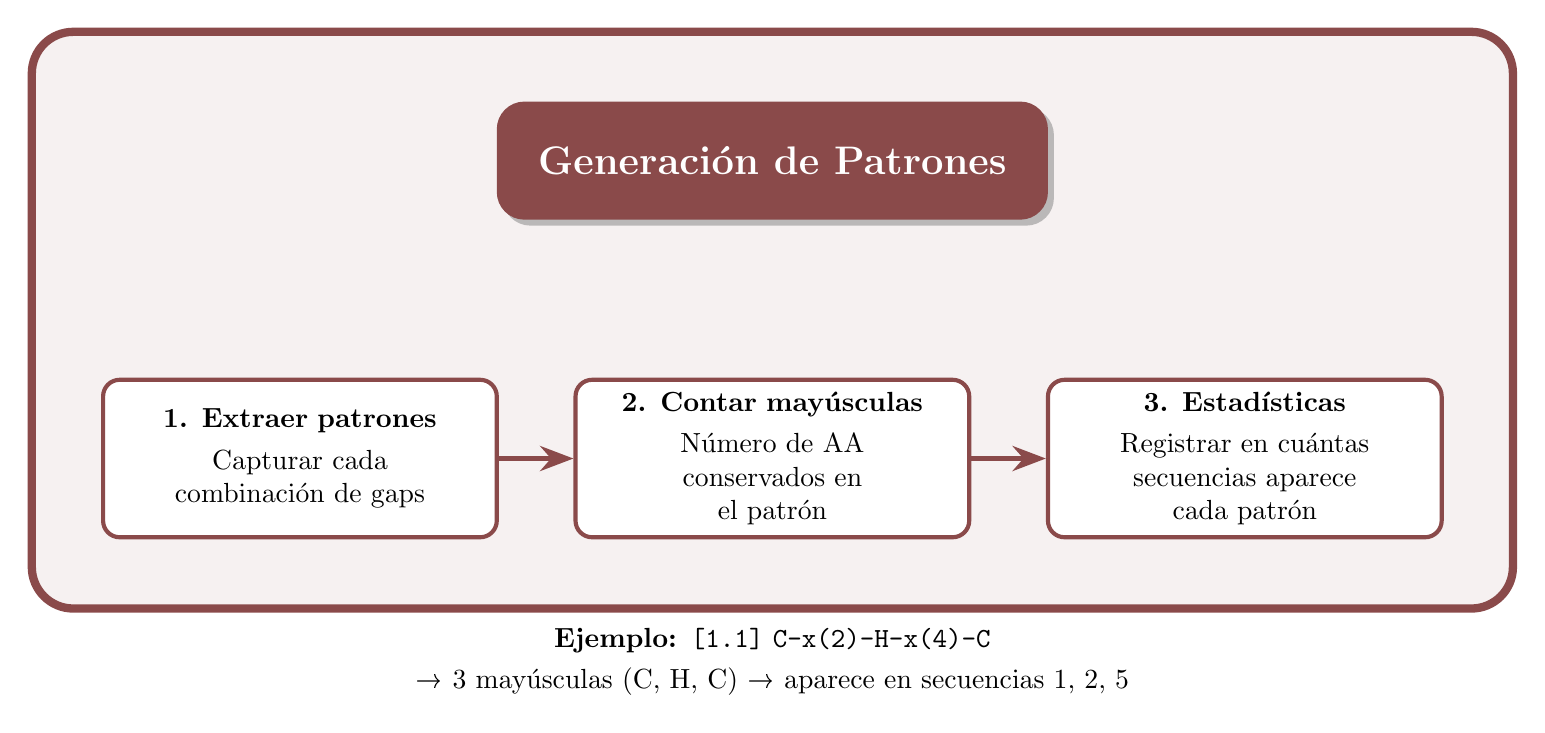
\begin{tikzpicture}[
        node distance=1.5cm,
        % Estilos para nodos principales
        mainbox/.style={
                rectangle,
                rounded corners=10pt,
                minimum width=7cm,
                minimum height=1.5cm,
                text centered,
                text width=6.5cm,
                font=\bfseries\Large,
                text=white,
                drop shadow
            },
        % Estilos para sub-nodos
        subbox/.style={
                rectangle,
                rounded corners=6pt,
                minimum width=5cm,
                minimum height=2cm,
                text centered,
                text width=4.5cm,
                font=\normalsize,
                text=black,
                fill=white,
                draw=FormalRed,
                line width=1.5pt
            },
        % Flechas
        arrow/.style={
                ->,
                >=Stealth,
                line width=2pt,
            color=FormalRed
            },
        % Grupo contenedor
        groupbox/.style={
                rectangle,
                rounded corners=15pt,
            draw=FormalRed,
                line width=3pt,
            fill=FormalRed!8,
                inner sep=25pt
            }
    ]

    % Título principal
    \node[mainbox, fill=FormalRed] (reconstruccion) {Generación de Patrones};

    % Sub-nodos
    \node[subbox, below=2cm of reconstruccion, xshift=-6cm] (rec1) {
        \textbf{1. Extraer patrones}\\[3pt]
        Capturar cada\\
        combinación de gaps
    };

    \node[subbox, below=2cm of reconstruccion] (rec2) {
        \textbf{2. Contar mayúsculas}\\[3pt]
        Número de AA\\
        conservados en\\
        el patrón
    };

    \node[subbox, below=2cm of reconstruccion, xshift=6cm] (rec3) {
        \textbf{3. Estadísticas}\\[3pt]
        Registrar en cuántas\\
        secuencias aparece\\
        cada patrón
    };

    % Grupo
    \begin{scope}[on background layer]
        \node[groupbox, fit=(reconstruccion)(rec1)(rec2)(rec3)] (grec) {};
    \end{scope}

    % Flechas entre sub-nodos
    \draw[arrow] (rec1.east) -- (rec2.west);
    \draw[arrow] (rec2.east) -- (rec3.west);

    % Ejemplo
    \node[below=1cm of rec2, text width=14cm, align=center, font=\normalsize] (ejemplo) {
        \textbf{Ejemplo:} \texttt{[1.1] C-x(2)-H-x(4)-C}\\[3pt]
        → 3 mayúsculas (C, H, C) → aparece en secuencias 1, 2, 5
    };

\end{tikzpicture}

\end{document}
